\chapter{Θεωρητικό υπόβαθρο}

Σε μια σκήνη τριών διαστάσεων, κάθε αντικείμενο ορίζεται από ένα σύνολο επιφανειών, σχηματίζοντας ένα κλειστό σύνολο γύρω από το εσωτερικό του αντικειμένου. Ωστόσο, υπάρχει ανάγκη για προβολή των εσωτερικών στοιχείων ή όψεων των τομών ενός αντικειμένου και για επεξεργασία της περιγραφής των αντικειμένων, προβάλλοντας μια καθορισμένη όψη τους πάνω στην επιφάνεια μιας συσκευής παρουσίασης. Συνεπώς, συγκριτικά με τη διδιάστατη απεικόνιση, η μεταφορά της σκηνής σε μια προβολή πάνω σε μια επίπεδη επιφάνεια απαιτεί τον εντοπισμό των ορατών τμημάτων μιας σκηνής, καθώς και τον υπολογισμό των εφέ φωτισμού και των χαρακτηριστικών των επιφανειών. \par

Η λήψη μιας προβολής 3Δ σκηνής παγκοσμίων συντεταγμένων απαιτεί και τον ορισμό αναφοράς συντεταγμένων θέασης. Αυτή ορίζει τη θέση και τον προσανατολισμό ενός επιπέδου θέασης, το οποίο αντιστοιχεί στο επίπεδο ενός φανταστικού φιλμ μιας κάμερας. Στη συνέχεια, οι περίγραφες των αντικειμένων μεταφέρονται στις συντεταγμένες αναφοράς θέασης σε μορφή περιγράμματος ή με την εφαρμογή τεχνικών φωτισμού και απόδοσης. Γενικώς, κατά τον μετασχηματισμό προβολής δεν διατηρούνται οι αναλογίες των αποστάσεων (\textlatin{Hearn \& Baker}, 2010, σ. 331). \par

Όσον αφορά την προβολή, αυτή δύναται να οριστεί ως η δημιουργία της εικόνας ενός αντικειμένου πάνω σε ένα απλούστερο αντικείμενο\footnote{Το απλούστέρο αντικείμενο προβολής είναι το επίπεδο ή μια επιφάνεια.}. Οι ευθείες προβολών ορίζονται από το κέντρο προβολής και τα προβαλλόμενα σημεία. Σε μια 3Δ σκηνή δύνανται να επιλεχθούν διαφορετικές μέθοδοι προβολής της σκηνής πάνω στο επίπεδο θέασης. Τα είδη των προβολών χωρίζονται σε παράλληλες προβολές (\textlatin{parallel projections}) και προοπτικές προβολές (\textlatin{perspective projections}). Ειδικώς, παράλληλη ονομάζεται η προβολή κατά την οποία τα σημεία της επιφάνειας του αντικειμένου προβάλλονται κατά μήκος παραλλήλων γραμμών και κύριο χαρακτηριστικό της είναι η ακριβής προβολή των διαστάσεων του προβαλλόμενου αντικειμένου, ενώ προοπτική ονομάζεται η προβολή κατά την οποία τα σημεία της επιφάνειας ενός αντικειμένου προβάλλονται κατά μήκος ιχνών που συγκλίνουν. Κύριο χαρακτηριστικό της τελευταίας είναι η ρεαλιστικότατά της (Μουστάκας κ.ά., 2015? \textlatin{Hearn \& Baker}, 2010). \par

Περεταίρω διαχωρισμός των δύο βασικών κατηγοριών προβολών δύναται να είναι ο απεικονιζόμενος εις την ακόλουθη εικόνα. \par

\begin{figure}[h]
\centering
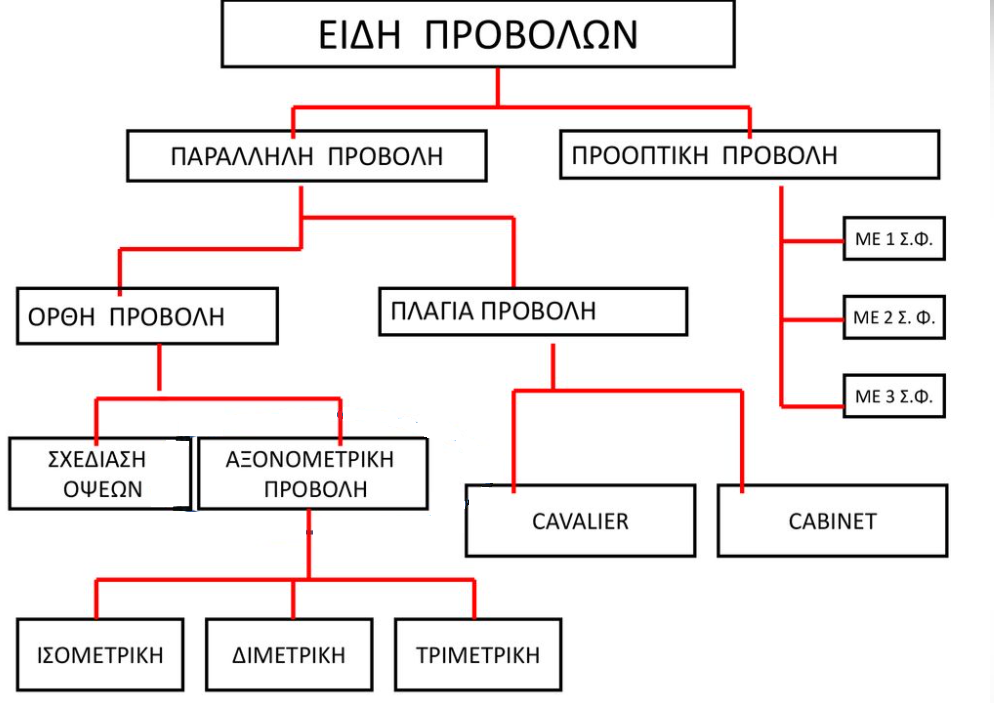
\includegraphics[width=0.75\textwidth]{images/projection}
\caption{Είδη προβολών}
\end{figure}

\hspace{0.5em}

Παρατηρώντας το παραπάνω σχήμα, διαπιστώνεται πως οι πλάγιες προβολές, το αντικείμενο ανάλυσης της παρούσας εργασίας, είναι υποκατηγορία των παραλλήλων προβολών. Γενικώς, πλάγια παράλληλη προβολή ονομάζεται η χαρτογράφηση κατά την οποία το ίχνος προβολής δεν είναι κάθετο στο επίπεδο θέασης. Οι πλάγιες προβολές ορίζονται από τη διεύθυνση ενός διανύσματος για τις γραμμές προβολής. \par

Δύο σημαντικές περιπτώσεις πλάγιας προβολής σε σχεδιαστικές εφαρμογές, όπως βλέπουμε και στην Eικόνα 1.1, αποτελούν οι \textlatin{Cavalier} με γωνία ύψους $45\degree$ και \textlatin{Cabinet} με γωνία ύψους $63\degree$. Προβολές \textlatin{Cavalier} ονομάζονται οι όψεις που λαμβάνουμε όταν η γωνία $a = 45\degree$ με $\tan a = 1$, όπου όλες οι γραμμές κάθετες του επιπέδου προβολής προβάλλονται χωρίς αλλαγή στο μήκος, ενώ προβολές \textlatin{Cabinet} χαρακτηρίζονται οι όψεις λαμβανόμενες για γωνία  $a = 63\degree$ με $\tan a = 2$. Σε αυτή την περίπτωση, οι γραμμές παράλληλες στην επιφάνεια θέασης προβάλλονται στο μισό του μήκους τους με αποτέλεσμα να φαίνονται πιο ρεαλιστικές εξαιτίας της μείωσης των καθέτων. \par

Στην ακόλουθη εικόνα απεικονίζεται παράδειγμα προβολής \textlatin{Cavalier} κύβου πάνω σε ένα επίπεδο θέασης για δύο τιμές της γωνίας $φ$, όπου το βάθος του κύβου προβάλλεται με μήκος ίσο με αυτό του πλάτους και του ύψους, καθώς και παράδειγμα προβολής \textlatin{Cabinet} κύβου πάνω σε ένα επίπεδο θέασης για δύο τιμές της γωνίας $φ$, όπου το βάθος προβάλλεται με μήκος μισό του πλάτους και του ύψους του κύβου (Σπύρου, 2019? \textlatin{Hearn \& Baker}, 2010). \par

\begin{figure}[h]
\centering
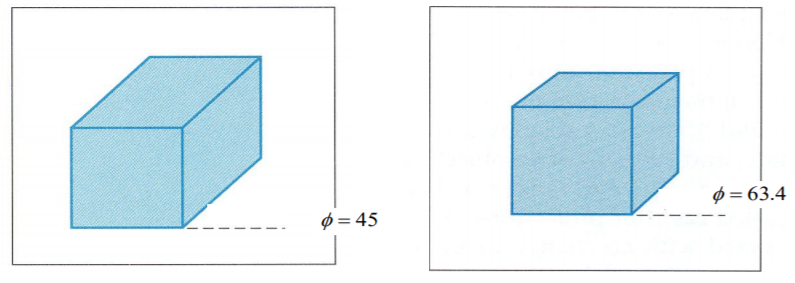
\includegraphics[width=0.75\textwidth]{images/projectionCabinet-Cavalier}
\caption{Παράδειγμα πλαγίων προβολών \textlatin{Cavalier}-\textlatin{Cabinet} }
\end{figure}